\documentclass{beamer}
\usepackage[utf8]{inputenc}
\usepackage[czech]{babel}
\usepackage{times}
\usepackage[T1]{fontenc}
\usepackage[ruled,longend,linesnumbered]{algorithm2e}
\usepackage{breakurl}

\title{
    Typografie a publikování\\
    \medskip
    Pátý projekt\\
    \bigskip
    \small{Dijkstrův algoritmus}
}
\author{
    Pavel Bobčík\\
    \small{xbobci03}
}
\date{1. května 2020}

\begin{document}

\maketitle
\begin{frame}
    \frametitle{Úvod do grafových algoritmů}
    \begin{itemize}[<+->]
        \item Slouží jako grafický způsob vyjádření vztahů mezi objekty.
        \item Objekty jsou reprezentovány \textbf{vrcholy}.
        \item \textbf{Hrany} reprezentují vztahy.
        \item Vztah mezi dvěma vrcholy vyznačíme jejich propojením pomocí hrany.
        \item Hrana musí být \textbf{vždy} zakončena. Ať už v druhém vrcholu, tak i sama v sobě.
        \begin{itemize}
            \item Taková hrana se nazývá \textbf{smyčka}.
        \end{itemize}
    \end{itemize}
\end{frame}

\begin{frame}
    \frametitle{Dijkstrův algoritmus - Definice}
    \begin{itemize}[<+->]
        \item Nejrychlejší známý algoritmus.
        \item Slouží k nalezení nejkratší cesty v grafu.
        \item Funguje u hranově (kladně) hodnoceného grafu.
        \item Je konečný. 
        \begin{itemize}
            \item Průchodů cyklem je nejvýše tolik, kolik má graf vrcholů.
        \end{itemize}
        \item Složitost je $O(|V|^2 + |E|)$.
        \begin{itemize}
            \item |V| představuje počet \textbf{vrcholů}.
            \item |E| představuje počet \textbf{hran}.
        \end{itemize}
        \item Vzdálenost mezi vrcholy grafu se počítá jako součet vzdálenosti aktuálního vrcholu od počátku a délka hrany k zpracovávanému vrcholu.
    \end{itemize}
\end{frame}

\begin{frame}
    \frametitle{Dijkstrův algoritmus - příklad}
    \begin{columns}
        \column{.5\textwidth}
        \only<1>{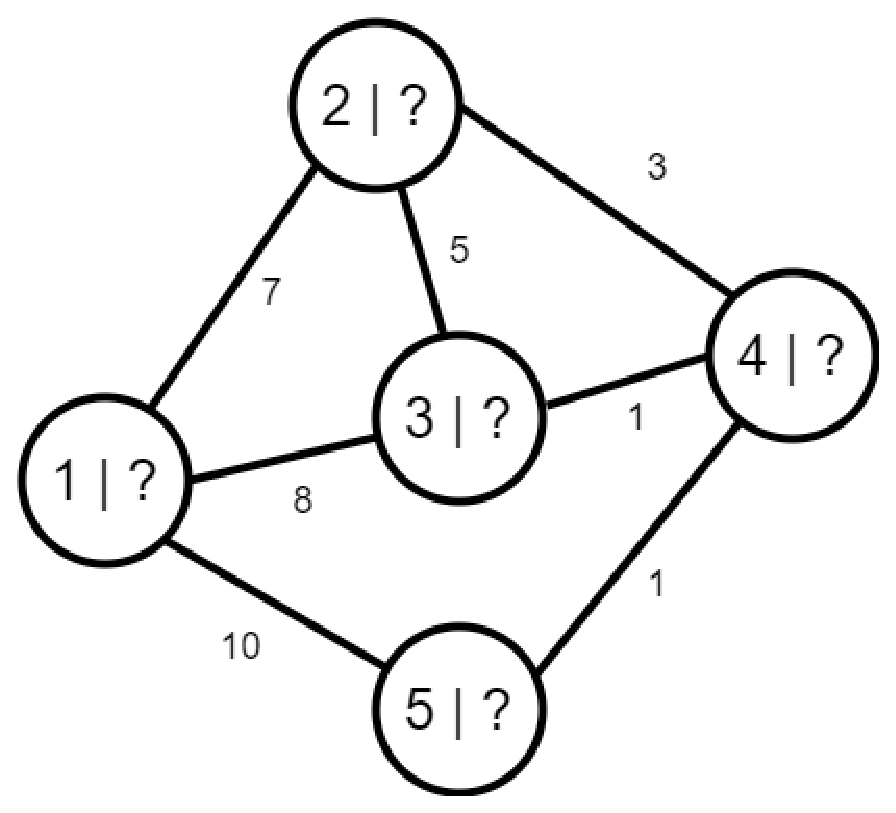
\includegraphics[scale=0.3]{dijk_01.eps}}
        \column{.5\textwidth}
        \begin{block}{Popis}
            \begin{itemize}
            \item V příkladu můžeme vidět:
            \begin{itemize}
                \item 5 vrcholů,
                \item 7 hran.
            \end{itemize}
            \end{itemize}
        \end{block}
    \end{columns}
\end{frame}

\begin{frame}
    \frametitle{Dijkstrův algoritmus - postup}
    \begin{columns}
        \column{.5\textwidth}
        \only<1>{\includegraphics[scale=0.3]{dijk_02.eps}}
        \column{.5\textwidth}
        \begin{block}{Popis}
            \begin{itemize}
                \item Vybranému vrcholu (pro nás vrchol 1) nastavíme vzdálenost 0.
            \end{itemize}
        \end{block}
        \begin{block}{Vrcholy}
            \begin{itemize}
                \item \textbf{Sousední:} 2; 3; 5 
                \item \textbf{K prohledání:} 1
            \end{itemize}
        \end{block}
    \end{columns}
\end{frame}

\begin{frame}
    \frametitle{Dijkstrův algoritmus - postup}
    \begin{columns}
        \column{.5\textwidth}
        \only<1>{\includegraphics[scale=0.3]{dijk_03.eps}}
        \column{.5\textwidth}
        \begin{block}{Popis}
            \begin{itemize}
                \item Vybereme nejkratší hranu, tedy k vrcholu 2.
                \item Získaná hodnota 7 (počáteční vrchol + hodnota hrany) je nižší, než původní (např. lze brát jako nekonečno).
            \end{itemize}
        \end{block}
        \begin{block}{Vrcholy}
            \begin{itemize}
                \item \textbf{Sousední:} 2; 3; 5 
                \item \textbf{K prohledání:} 2
            \end{itemize}
        \end{block}
    \end{columns}
\end{frame}

\begin{frame}
    \frametitle{Dijkstrův algoritmus - postup}
    \begin{columns}
        \column{.5\textwidth}
        \only<1>{\includegraphics[scale=0.3]{dijk_04.eps}}
        \column{.5\textwidth}
        \begin{block}{Popis}
            \begin{itemize}
                \item Nyní prozkoumáme hranu k vrcholu 3.
                \item Získaná hodnota 8 je nižší, než původní (nekonečno).
            \end{itemize}
        \end{block}
        \begin{block}{Vrcholy}
            \begin{itemize}
                \item \textbf{Sousední:} 2; 3; 5 
                \item \textbf{K prohledání:} 2; 3
            \end{itemize}
        \end{block}
    \end{columns}
\end{frame}

\begin{frame}
    \frametitle{Dijkstrův algoritmus - postup}
    \begin{columns}
        \column{.5\textwidth}
        \only<1>{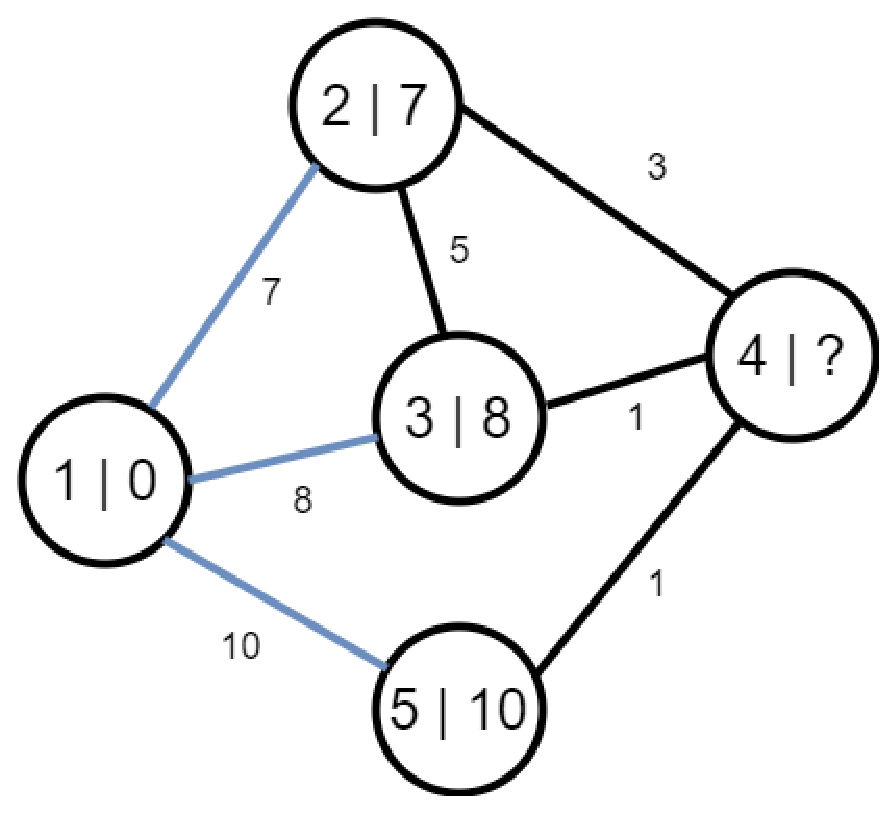
\includegraphics[scale=0.3]{dijk_05.eps}}
        \column{.5\textwidth}
        \begin{block}{Popis}
            \begin{itemize}
                \item Jako poslední hrana jdoucí z vrcholu 1 je hrana k vrcholu 5.
                \item Získaná hodnota 10 je nižší, než původní (nekonečno).
            \end{itemize}
        \end{block}
        \begin{block}{Vrcholy}
            \begin{itemize}
                \item \textbf{Sousední:} 2; 3; 5 
                \item \textbf{K prohledání:} 2; 3; 5
            \end{itemize}
        \end{block}
    \end{columns}
\end{frame}

\begin{frame}
    \frametitle{Dijkstrův algoritmus - postup}
    \begin{columns}
        \column{.5\textwidth}
        \only<1>{\includegraphics[scale=0.3]{dijk_06.eps}}
        \column{.5\textwidth}
        \begin{block}{Popis}
            \begin{itemize}
                \item Nyní již máme vrchol 1 kompletní, přestoupíme tedy na vrchol dva.
            \end{itemize}
        \end{block}
        \begin{block}{Vrcholy}
            \begin{itemize}
                \item \textbf{Sousední:} 3; 4 
                \item \textbf{K prohledání:} 2
            \end{itemize}
        \end{block}
    \end{columns}
\end{frame}

\begin{frame}
    \frametitle{Dijkstrův algoritmus - postup}
    \begin{columns}
        \column{.5\textwidth}
        \only<1>{\includegraphics[scale=0.3]{dijk_07.eps}}
        \column{.5\textwidth}
        \begin{block}{Popis}
            \begin{itemize}
                \item Prozkoumáme hranu k vrcholu 3.
                \item Součet hodnoty vrcholu dva a hrany nám vrátí 12. Tato hodnota je vyšší, cestu tedy neměníme.
            \end{itemize}
        \end{block}
        \begin{block}{Vrcholy}
            \begin{itemize}
                \item \textbf{Sousední:} 3; 4 
                \item \textbf{K prohledání:} 3
            \end{itemize}
        \end{block}
    \end{columns}
\end{frame}

\begin{frame}
    \frametitle{Dijkstrův algoritmus - postup}
    \begin{columns}
        \column{.5\textwidth}
        \only<1>{\includegraphics[scale=0.3]{dijk_08.eps}}
        \column{.5\textwidth}
        \begin{block}{Popis}
            \begin{itemize}
                \item Nyní prozkoumáme hranu k vrcholu 4.
                \item Hodnota se rovná 10, což je lepší než nekonečno. Vznikla nám tedy nová cesta.
            \end{itemize}
        \end{block}
        \begin{block}{Vrcholy}
            \begin{itemize}
                \item \textbf{Sousední:} 1; 3; 4 
                \item \textbf{K prohledání:} 3; 4
            \end{itemize}
        \end{block}
    \end{columns}
\end{frame}

\begin{frame}
    \frametitle{Dijkstrův algoritmus - postup}
    \begin{columns}
        \column{.5\textwidth}
        \only<1>{\includegraphics[scale=0.3]{dijk_09.eps}}
        \column{.5\textwidth}
        \begin{block}{Popis}
            \begin{itemize}
                \item Vyřešili jsme druhý vrchol.
                \item Nyní si jej můžeme označit jako hotový a přestoupit na vrchol 3.
            \end{itemize}
        \end{block}
        \begin{block}{Vrcholy}
            \begin{itemize}
                \item \textbf{Sousední:} 1; 2; 4 
                \item \textbf{K prohledání:} 3
            \end{itemize}
        \end{block}
    \end{columns}
\end{frame}

\begin{frame}
    \frametitle{Dijkstrův algoritmus - postup}
    \begin{columns}
        \column{.5\textwidth}
        \only<1>{\includegraphics[scale=0.3]{dijk_10.eps}}
        \column{.5\textwidth}
        \begin{block}{Popis}
            \begin{itemize}
                \item Cesta z třetího do druhého vrcholu je delší, než již existující. Cestu tedy ponecháme.
            \end{itemize}
        \end{block}
        \begin{block}{Vrcholy}
            \begin{itemize}
                \item \textbf{Sousední:} 1; 2; 4 
                \item \textbf{K prohledání:} 
            \end{itemize}
        \end{block}
    \end{columns}
\end{frame}

\begin{frame}
    \frametitle{Dijkstrův algoritmus - postup}
    \begin{columns}
        \column{.5\textwidth}
        \only<1>{\includegraphics[scale=0.3]{dijk_11.eps}}
        \column{.5\textwidth}
        \begin{block}{Popis}
            \begin{itemize}
                \item Můžeme vyznačit hranu mezi vrcholy 1. a 2. jako hotovou, protože jsme našli nejkratší cestu.
            \end{itemize}
        \end{block}
        \begin{block}{Vrcholy}
            \begin{itemize}
                \item \textbf{Sousední:} 1; 2; 4 
                \item \textbf{K prohledání:} 
            \end{itemize}
        \end{block}
    \end{columns}
\end{frame}

\begin{frame}
    \frametitle{Dijkstrův algoritmus - postup}
    \begin{columns}
        \column{.5\textwidth}
        \only<1>{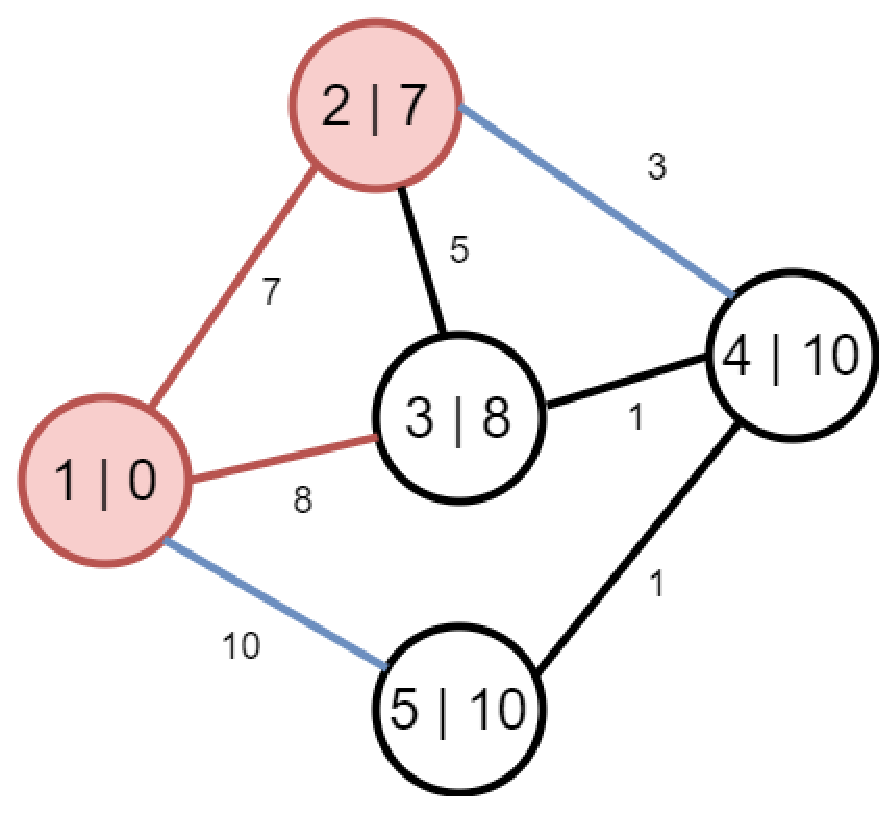
\includegraphics[scale=0.3]{dijk_12.eps}}
        \column{.5\textwidth}
        \begin{block}{Popis}
            \begin{itemize}
                \item Rovněž můžeme vyznačit i~hranu mezi 1. a 2. vrcholem jako nejkratší cestu.
            \end{itemize}
        \end{block}
        \begin{block}{Vrcholy}
            \begin{itemize}
                \item \textbf{Sousední:} 1; 2; 4 
                \item \textbf{K prohledání:} 
            \end{itemize}
        \end{block}
    \end{columns}
\end{frame}

\begin{frame}
    \frametitle{Dijkstrův algoritmus - postup}
    \begin{columns}
        \column{.5\textwidth}
        \only<1>{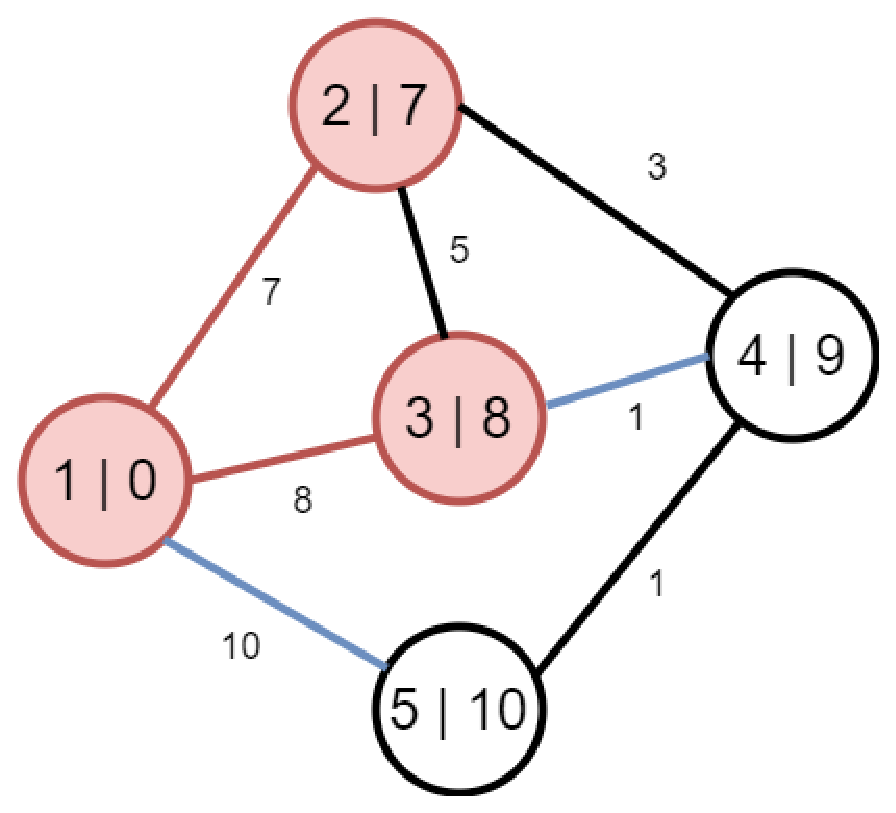
\includegraphics[scale=0.3]{dijk_13.eps}}
        \column{.5\textwidth}
        \begin{block}{Popis}
            \begin{itemize}
                \item Prozkoumáme zbývající cestu a to k 4. vrcholu.
                \item Jelikož se nám zlepšila vzdálenost k 4. vrcholu, přepíšeme stávající hodnotu novou.
                \item Nyní můžeme i 3. vrchol označit jako hotový.
            \end{itemize}
        \end{block}
        \begin{block}{Vrcholy}
            \begin{itemize}
                \item \textbf{Sousední:} 1; 2; 4 
                \item \textbf{K prohledání:} 4
            \end{itemize}
        \end{block}
    \end{columns}
\end{frame}

\begin{frame}
    \frametitle{Dijkstrův algoritmus - postup}
    \begin{columns}
        \column{.5\textwidth}
        \only<1>{\includegraphics[scale=0.3]{dijk_14.eps}}
        \column{.5\textwidth}
        \begin{block}{Popis}
            \begin{itemize}
                \item Nyní zjistíme cestu ze 4. do 5. vrcholu.
                \item Můžeme si všimnout, že se nemění vzdálenost, ponecháme tedy původní.
                \item Cestu lze i změnit, výsledná hodnota se nám nijak nezmění. Pozmění se pouze vykreslení grafu.
            \end{itemize}
        \end{block}
        \begin{block}{Vrcholy}
            \begin{itemize}
                \item \textbf{Sousední:} 3; 5
                \item \textbf{K prohledání:} 
            \end{itemize}
        \end{block}
    \end{columns}
\end{frame}

\begin{frame}
    \frametitle{Dijkstrův algoritmus - výsledek}
    \begin{columns}
        \column{.5\textwidth}
        \only<1>{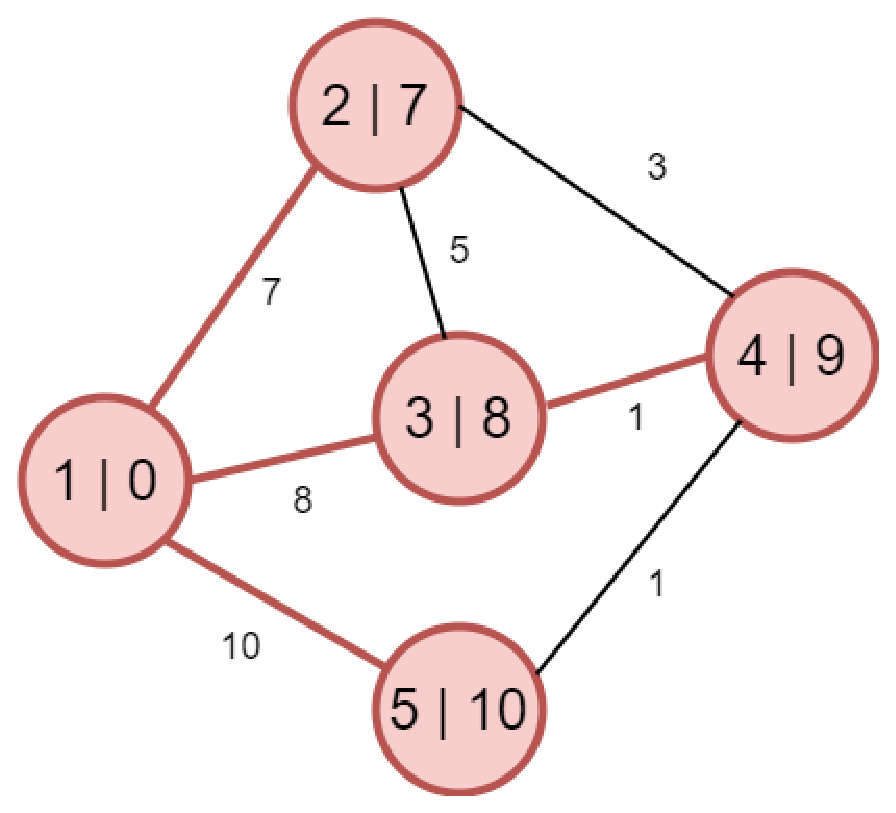
\includegraphics[scale=0.3]{dijk_15.eps}}
        \column{.5\textwidth}
        \begin{block}{Popis}
            \begin{itemize}
                \item Ve výsledku vidíme vyznačený průchod grafem po jeho nejkratších cestách.
                \item Všimněte si, že nám nevznikla smyčka. Pokud by se zde vyskytovala, tak jsme někde chybovali.
            \end{itemize}
        \end{block}
    \end{columns}
\end{frame}

\begin{frame}
    \frametitle{Použité zdroje}
    \begin{itemize}
        \item Tvorba grafu: \\ \small{\url{https://app.diagrams.net}}
        \item Vizuální popis Dijkstrova algoritmu: \\ \url{https://www.youtube.com/watch?v=J8Cce722fkY}
        \item Textová část: \\ \url{https://is.muni.cz/th/vszrq/xrbenkovsky.pdf} \\
        \url{https://cs.wikipedia.org/wiki/Dijkstrův_algoritmus} \\
        \url{https://www.algoritmy.net/article/5108/Dijkstruv-algoritmus} \\
        \url{https://phoenix.inf.upol.cz/esf/ucebni/Grafy_a_grafove_algoritmy.pdf}
    \end{itemize}
\end{frame}

\end{document}

